\documentclass[tikz,border=4pt]{standalone}
\usepackage{amsmath}
\begin{document}
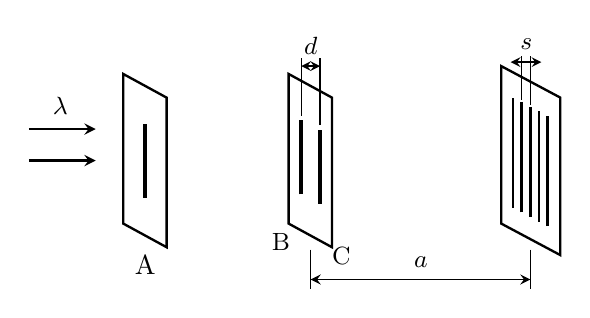
\begin{tikzpicture}[>=stealth, thick, scale=1.0]
  % Incident light arrows from left
  \draw[->, line width=0.8pt] (-1.2, 0.25) -- (-0.35, 0.25);
  \draw[->, line width=0.8pt] (-1.2, -0.15) -- (-0.35, -0.15);
  \node[above, font=\small] at (-0.8, 0.30) {$\lambda$};

  % Single slit A (tilted plate in perspective)
  \draw[line width=0.85pt] (0, -0.95) -- (0.55, -1.25) -- (0.55, 0.65) -- (0, 0.95) -- cycle;
  \draw[line width=1.4pt] (0.275, -0.62) -- (0.275, 0.32);
  \node[below] at (0.28, -1.22) {$\mathrm{A}$};

  % Double slit B, C (tilted plate)
  \draw[line width=0.85pt] (2.1, -0.95) -- (2.65, -1.25) -- (2.65, 0.65) -- (2.1, 0.95) -- cycle;
  \draw[line width=1.4pt] (2.26, -0.58) -- (2.26, 0.36);
  \draw[line width=1.4pt] (2.50, -0.70) -- (2.50, 0.24);
  \node[below left, font=\small] at (2.25, -0.95) {$\mathrm{B}$};
  \node[below right, font=\small] at (2.52, -1.12) {$\mathrm{C}$};

  % Slit spacing d dimension above B, C
  \draw[line width=0.5pt] (2.26, 0.42) -- (2.26, 1.15);
  \draw[line width=0.5pt] (2.50, 0.30) -- (2.50, 1.15);
  \draw[<->, line width=0.55pt] (2.26, 1.05) -- (2.50, 1.05);
  \node[above, font=\small] at (2.38, 1.07) {$d$};

  % Screen (tilted plate) with vertical fringes
  \draw[line width=0.85pt] (4.8, -0.95) -- (5.55, -1.35) -- (5.55, 0.65) -- (4.8, 1.05) -- cycle;
  \foreach \k in {0, 1, 2, 3, 4} {
    \draw[line width=0.9pt] ({4.95 + 0.11*\k}, {-0.75 - 0.058*\k}) -- ({4.95 + 0.11*\k}, {0.65 - 0.058*\k});
  }
  % Fringe spacing s dimension above screen
  \draw[line width=0.5pt] (5.06, 0.62) -- (5.06, 1.18);
  \draw[line width=0.5pt] (5.17, 0.56) -- (5.17, 1.18);
  \draw[<->, line width=0.55pt] (4.92, 1.10) -- (5.31, 1.10);
  \node[above, font=\small] at (5.12, 1.13) {$s$};

  % Distance a between double slit and screen
  \draw[line width=0.5pt] (2.38, -1.28) -- (2.38, -1.78);
  \draw[line width=0.5pt] (5.17, -1.28) -- (5.17, -1.78);
  \draw[<->, line width=0.6pt] (2.38, -1.66) -- (5.17, -1.66);
  \node[above, font=\small] at (3.78, -1.64) {$a$};
\end{tikzpicture}
\end{document}
